\section{Results}

In the following sections we will discuss some key results;
for a more complete look at the output of the scripts, we ask that you please
consult the \hyperref[apen]{Appendices}.

\subsection{Teleportation}

\begin{figure}[h!] \centering 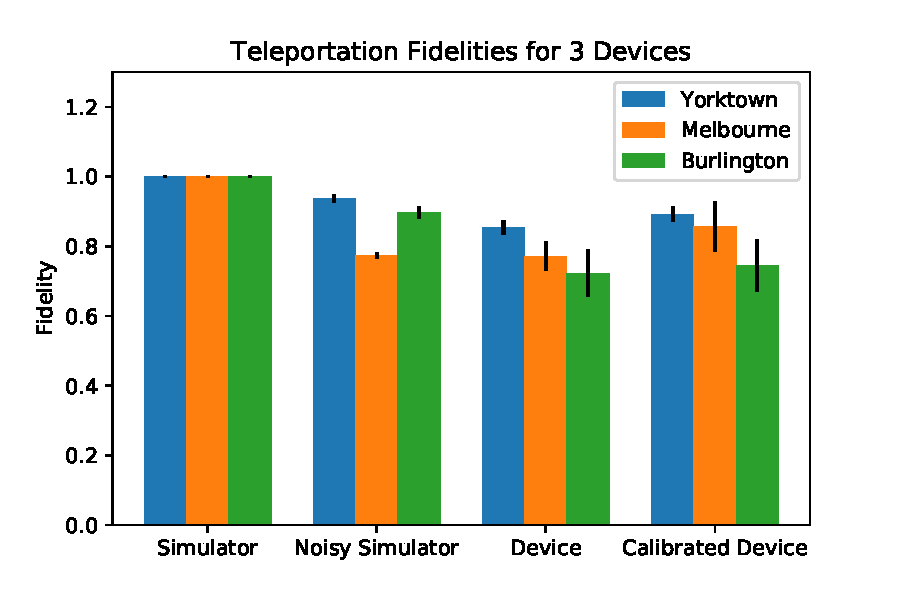
\includegraphics[width=0.48\textwidth]{images/results/teleport_histogram.pdf}
	\caption{Fidelity results for the Teleportation protocol. Error bars, showing
    one standard deviation, are estimated by taking the variance over 15 runs of
    8,192 shots each (a total of 122,880 shots). All simulation fidelities are
    within statistical error of unity.}
	\label{fig:teleport_histogram}
\end{figure}

The main result of the teleportation protocol is summarized in Fig.
\ref{fig:teleport_histogram}. The ideal simulation fidelities are all within
statistical error of unity, an important check to ensure that the state,
reconstructed through tomography and post-measurement selection scheme both are
working as expected.

\begin{figure}[h!]
  \begin{subfigure}{.5\textwidth}
    \centering
    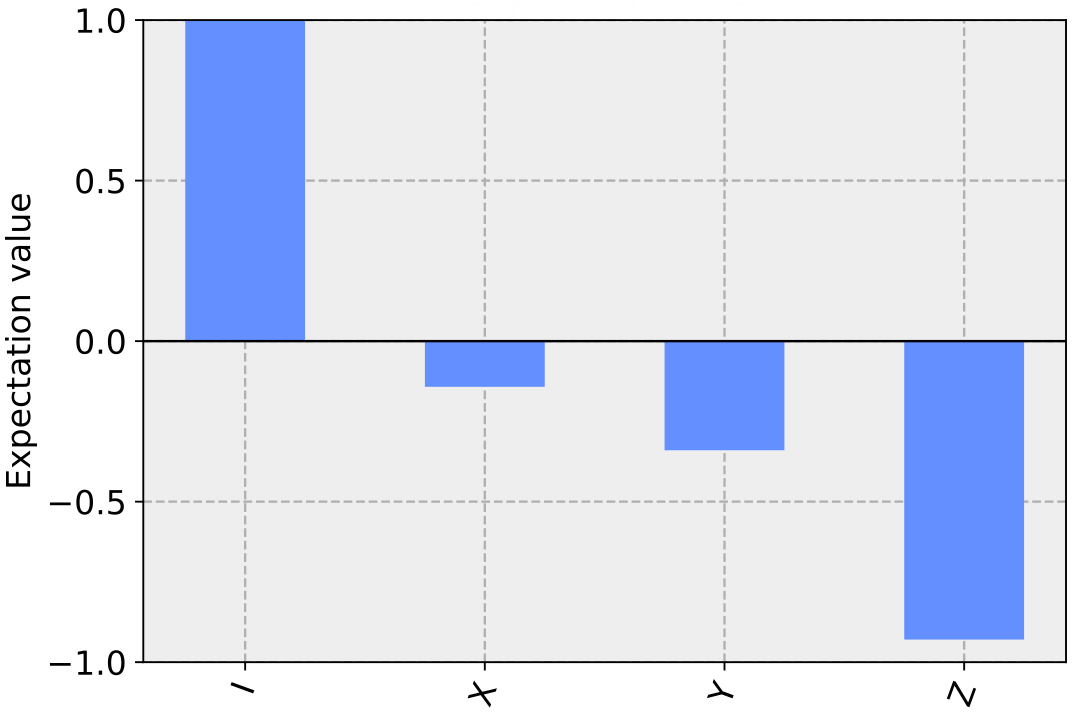
\includegraphics[width=.8\linewidth]{images/results/tele_pauli_sim.png}
    \caption{The expected Pauli set.}
    \label{fig:tele_pauli_sim}
  \end{subfigure}
  \newline
  \begin{subfigure}{.5\textwidth}
    \centering
    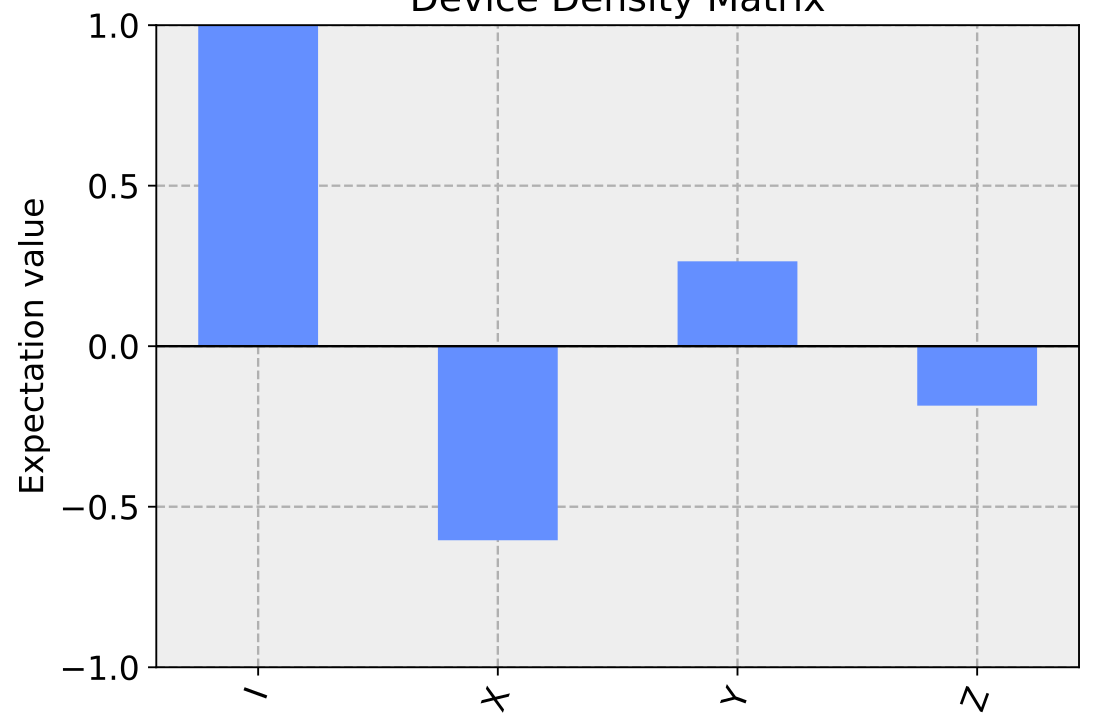
\includegraphics[width=.8\linewidth]{images/results/tele_pauli_dev.png}
    \caption{The output Pauli set for the device.}
    \label{fig:tele_pauli_dev}
  \end{subfigure}
  \newline
  \begin{subfigure}{.5\textwidth}
    \centering
    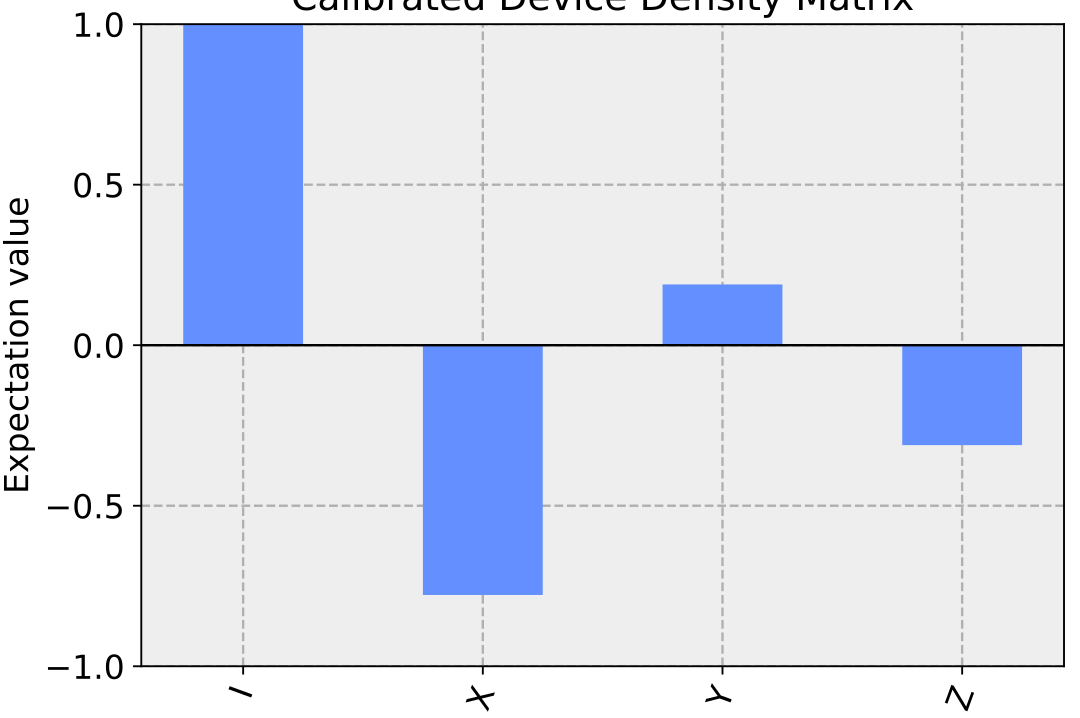
\includegraphics[width=.8\linewidth]{images/results/tele_pauli_cal.png}
    \caption{The calibrated device Pauli set.}
    \label{fig:tele_pauli_dev}
  \end{subfigure}
  \caption{The expectation values match those we expect after calibrating for
readout error. Errors in measurement contribute greatly to the low fidelity of
our final states. The type of correction seen in the figures above accounts for
the increased fidelity for the calibrated device in Fig.
\ref{fig:teleport_histogram}. Data plotted here is taken for 8192 shots on the
Melbourne backend.}
  \label{fig:tele_paulis}
\end{figure}

The Noisy Simulator is modelled using the single-qubit
errors, CNOT errors and a model of readout error with symmetric bit flip
probabilities in each backend \cite{qiskit_org}. As we will continue to see with
the other circuits, the noise model tends to overestimates the performance of
the backend, but interestingly in this case, for the Melbourne device, we find
that the noise model almost matches that of the device.

The noise model captures the error in the Burlington device much less
accurately. We would expect that Burlington would perform almost as well as
Yorktown from the estimates on the noisy simulator, but in fact it performs the
worst of the three. We suspect, as will be seen again below for the other
circuits, that this is a consequence of the number of gates needed to implement
the circuit on the real device.

\begin{figure}[h!]
  \centering
  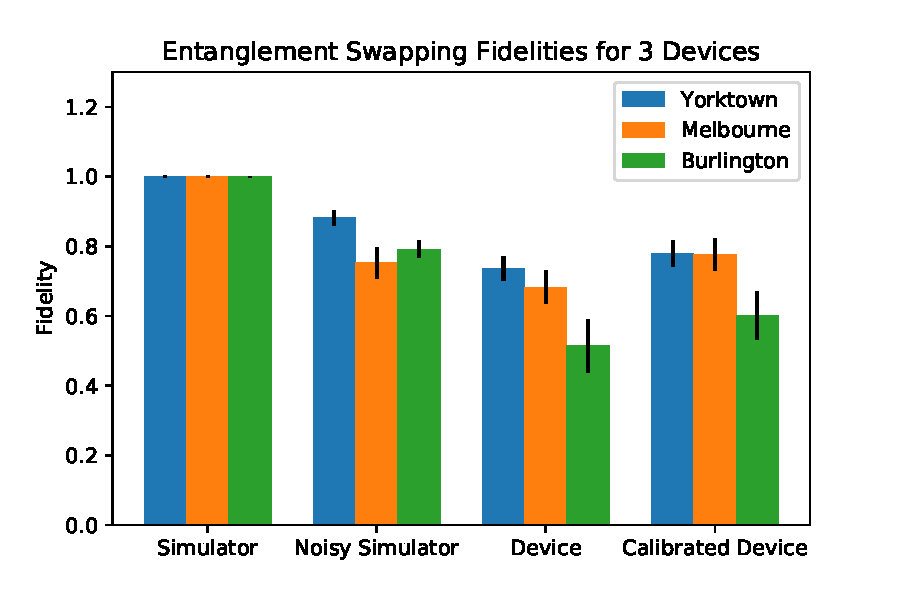
\includegraphics[width=0.48\textwidth]{images/results/swap_histogram.pdf}
	\caption{Fidelity results for the Entanglement Swapping protocol. Error bars
    are estimated by taking the variance over 15 runs of 8,192 shots each (a total
    of 122,880 shots).}
	\label{fig:swap_histogram}
\end{figure}

In order to check the readout calibration, it is useful to compare Pauli sets of
the different outcomes, which we can see in Fig. \ref{fig:tele_paulis}. These
plots make the expectation values of the three measurement bases very visible,
which eases the comparison of the results. Though not perfect, the output
calibrated for readout error fits the expected state much better than the
original device output. We can conclude from this that indeed, a large source of
error in the system comes from measurement, and the state the circuit actually
creates is much better than what we would naively assume through tomography
alone!

% This thing here is to test a full size picture don't delete.
% \begin{figure*}
%   \centering
%   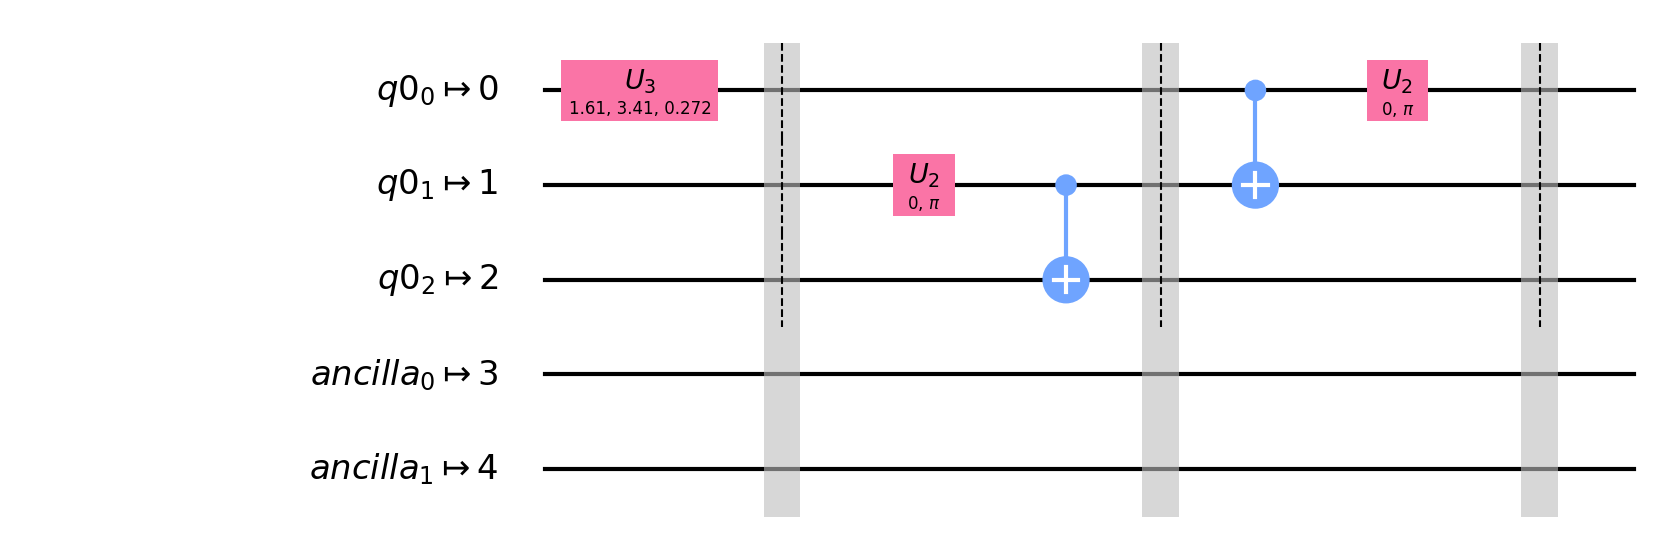
\includegraphics[width=\textwidth]{images/teleport_ibmqx2.png}
%   \caption{The most densely connected 5-qubit device at IBM Q. As we will see,
%     equally as important as the single-qubit and CNOT error rates is the degree of
%     connectivity in a device. Figure from \cite{ibmq_yorktown}.}
%   \label{fig:yorktown_connections}
% \end{figure*}

\subsection{Entanglement Swapping}

\begin{figure}[h!]
	\begin{subfigure}{.5\textwidth} \centering % include first image
		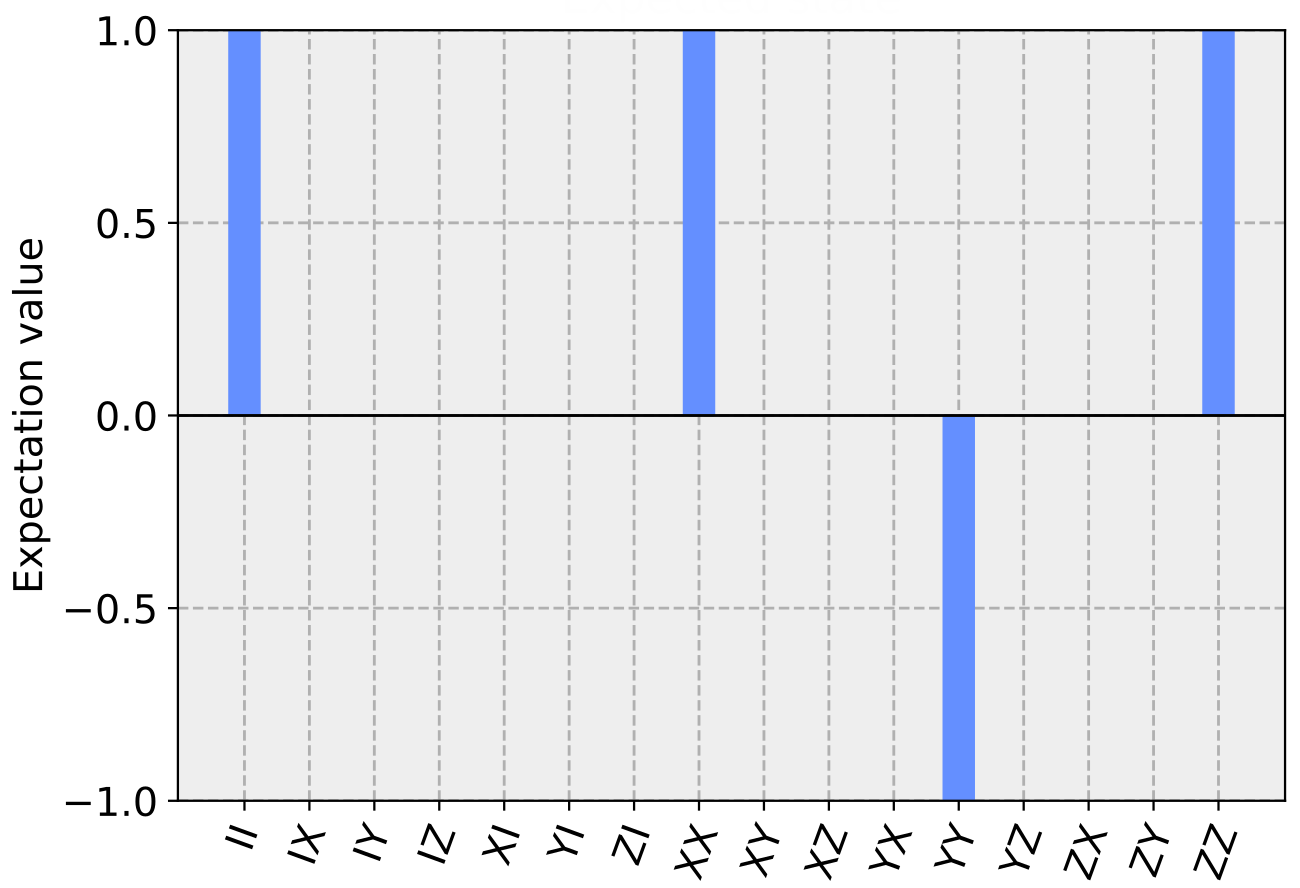
\includegraphics[width=.8\linewidth]{images/results/swap_pauli_sim.png}
		\caption{The expected Pauli set.}
		\label{fig:swap_pauli_sim}
	\end{subfigure} \newline
	\begin{subfigure}{.5\textwidth} \centering % include second image
		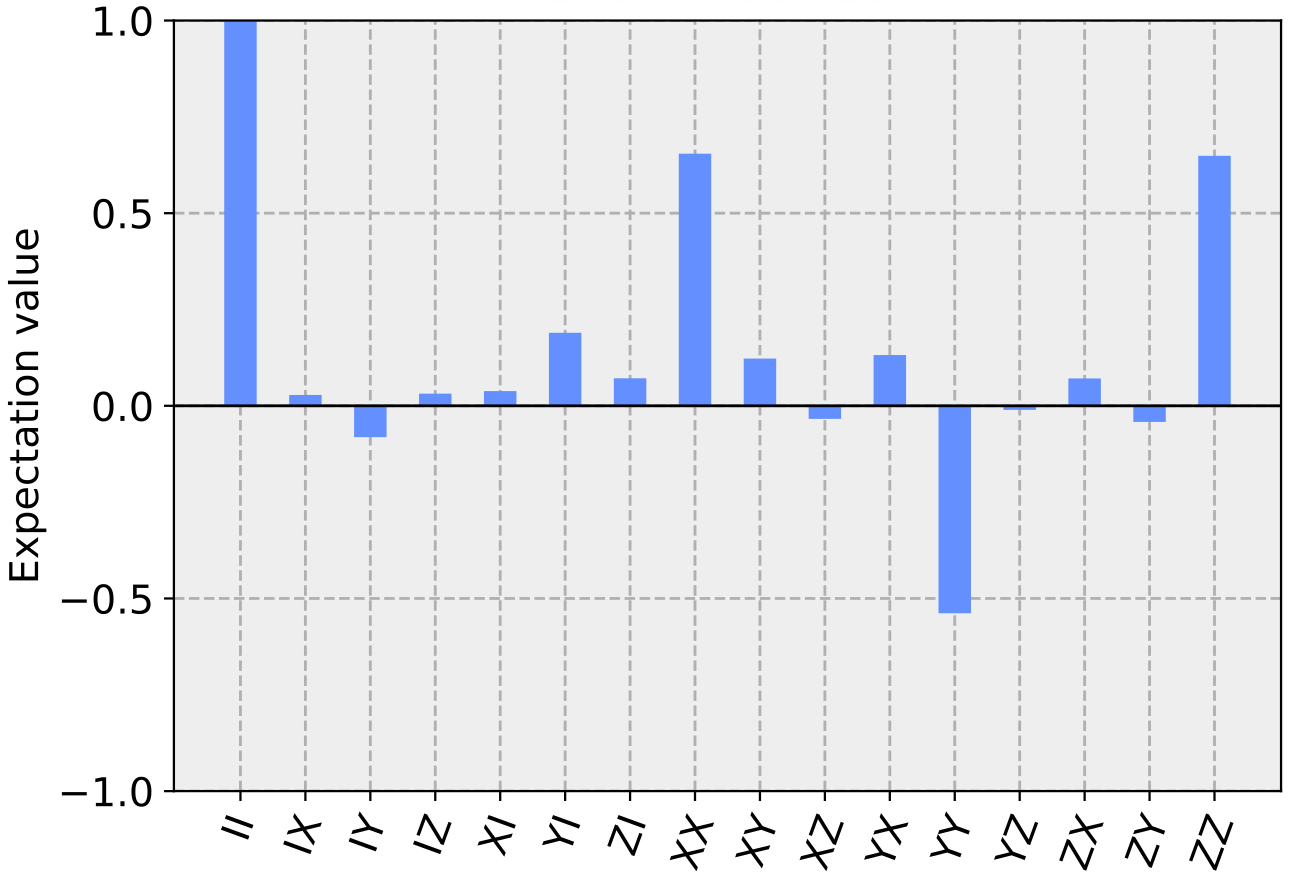
\includegraphics[width=.8\linewidth]{images/results/swap_pauli_dev.png}
		\caption{The output Pauli set for the device.}
		\label{fig:swap_pauli_dev}
	\end{subfigure} \newline
	\begin{subfigure}{.5\textwidth} \centering % include second image
		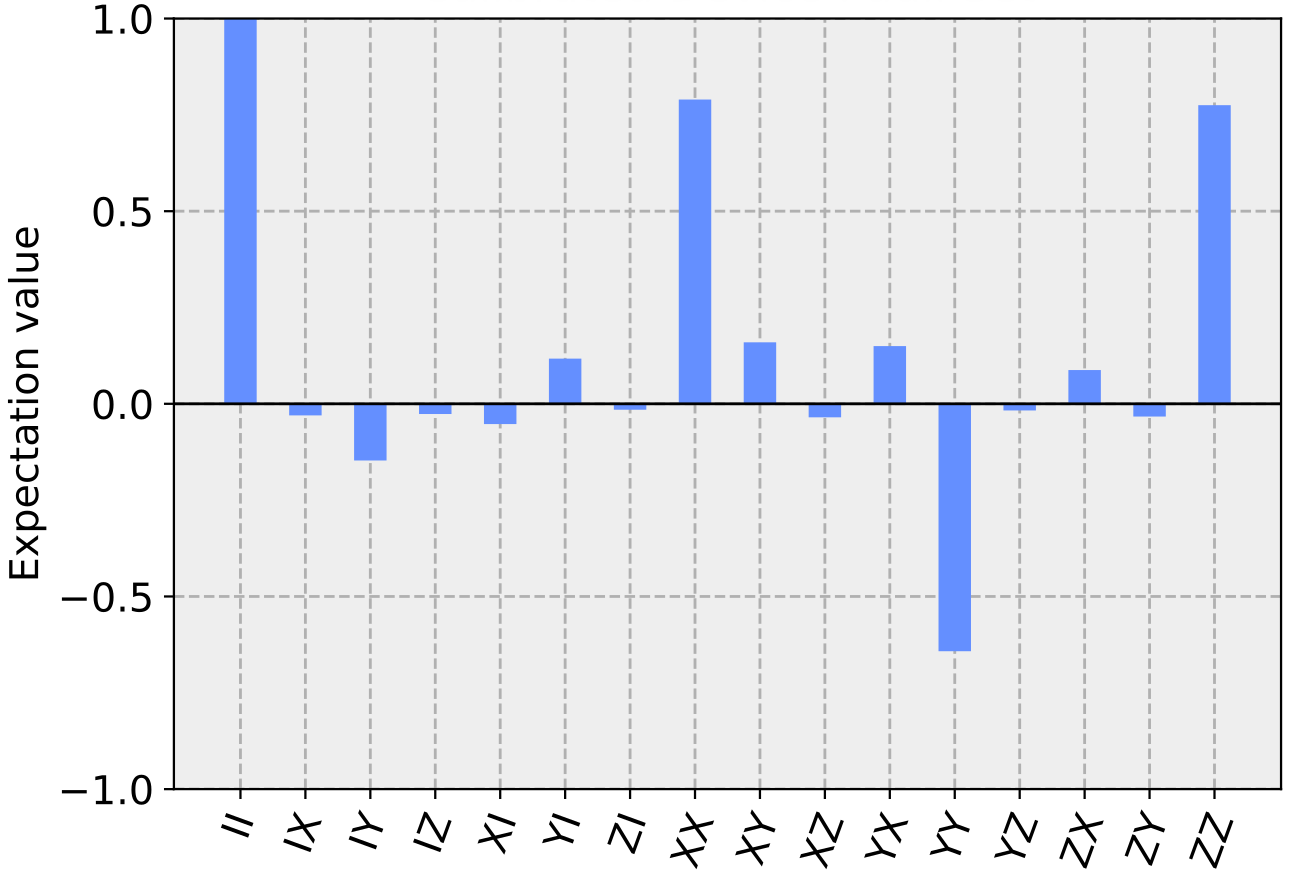
\includegraphics[width=.8\linewidth]{images/results/swap_pauli_cal.png}
		\caption{The calibrated device Pauli set.}
		\label{fig:swap_pauli_dev}
	\end{subfigure}
	\caption{Pauli set entanglement swapping results for the ideal simulator, the
		device and the calibrated device. The type of correction seen in the figures
		above accounts for the increased fidelity for the calibrated device in Fig.
		\ref{fig:swap_histogram}. Data plotted here is taken for 8192 shots on the
		Melbourne backend.}
	\label{fig:swap_paulis}
\end{figure} 

We now turn to Entanglement Swapping, a protocol largely similar to
teleportation, in that it teleports one half of an entangled pair. The main
result can be found in Fig. \ref{fig:swap_histogram}. The swapping protocol was
implemented for initial states (that is, the top two qubits, the bottom two were
always prepared in $\ket{\Phi^+}$) that were not, in general, Bell states, but
instead states with some degree of entanglement. We felt this was important in
order to probe our ability to reconstruct arbitrary states using tomography, and
show that indeed the swapping protocol should work for any entangled pair.

\begin{figure}[h]
	\begin{subfigure}{.5\textwidth}
    \centering
		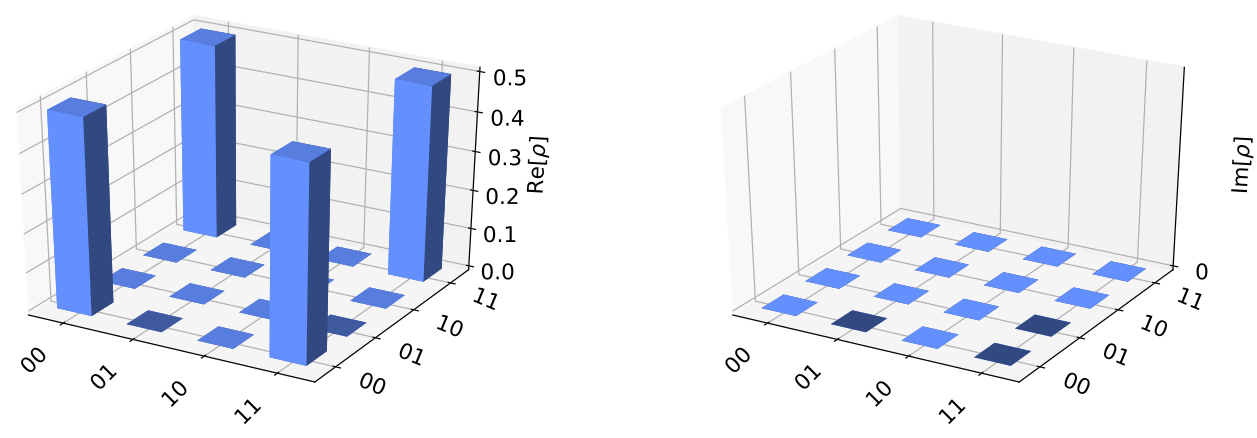
\includegraphics[width=.8\linewidth]{images/results/swap_density_sim.png}
		\caption{The expected Density matrix.}
		\label{fig:swap_density_sim}
	\end{subfigure} \newline
	\begin{subfigure}{.5\textwidth}
    \centering
		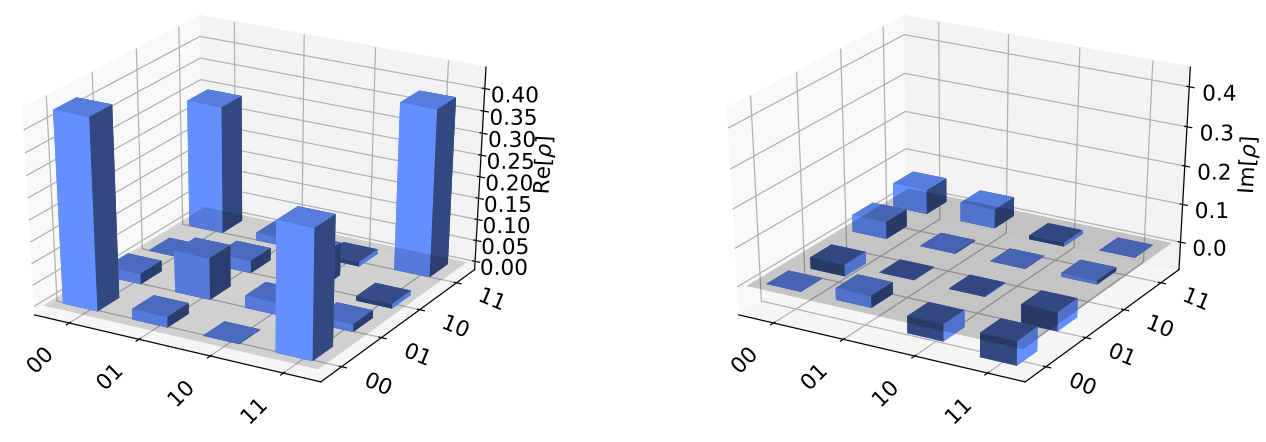
\includegraphics[width=.8\linewidth]{images/results/swap_density_dev.png}
		\caption{The output Density matrix for the device.}
		\label{fig:swap_density_dev}
	\end{subfigure} \newline
	\begin{subfigure}{.5\textwidth}
    \centering
		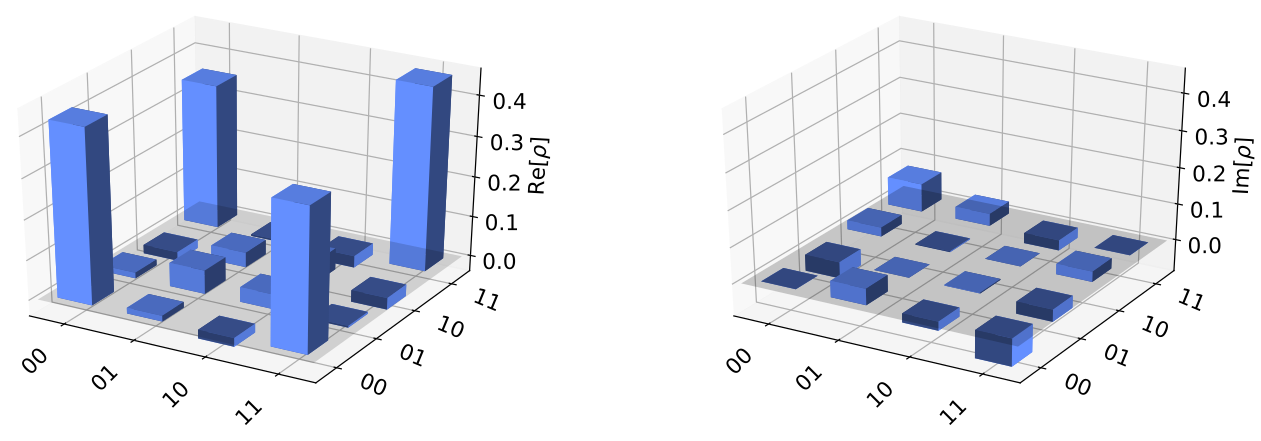
\includegraphics[width=.8\linewidth]{images/results/swap_density_cal.png}
		\caption{The calibrated device Density matrix.}
		\label{fig:swap_density_dev}
	\end{subfigure}
	\caption{The entanglement swapping density matrices for the ideal simulator,
    the device and the calibrated device. Data plotted here is taken for 8192 shots
    on the Melbourne backend. }
	\label{fig:swap_density}
\end{figure}

Again we see that the simulation fidelities are 1 within
statistical error, which means that the swapping of initial Bell-states are done
correctly using tomography to construct the final state, and post-measurement
selection to transform specified results to specific basis. As we expected,
fidelities from the noisy simulator are much better than results from all the
devices. Burlington's device performance is again much worse than would be
expected from the noisy simulator results. We can appreciate this decline by
comparing the number of gates needed to implement swap on Burlington to those
numbers for Melbourne and Yorktown. Where the former requires 9 CNOT gates to
implement the protocol on its T-shaped circuitry, the latter two require the
minimum of just three. This has huge impact on the output, and places the
backend with the highest single-qubit U$_2$ and CNOT fidelities in last place
when it comes to implementing swap.

In order to appreciate the effect of readout calibration on the output, we show,
in Fig. \ref{fig:swap_paulis}, the Pauli sets for an entanglement swapping
circuit that takes both input pairs as $\ket{\Phi^+}$. We chose this for our
plots as it is particularly easy, with a Bell state, to know what it is we
expect from the plots. 

We expect, of course, large values for the $\langle XX \rangle$, $\langle YY
\rangle$, $\langle ZZ \rangle$, and otherwise very small values, as seen in Fig.
\ref{fig:swap_pauli_sim}. The readout calibration does a decent job of boosting
the like-like correlations, as can also be seen from Fig.
\ref{fig:swap_density}.

\subsection{Entanglement Purification}

\begin{figure}[h!]
  \centering
  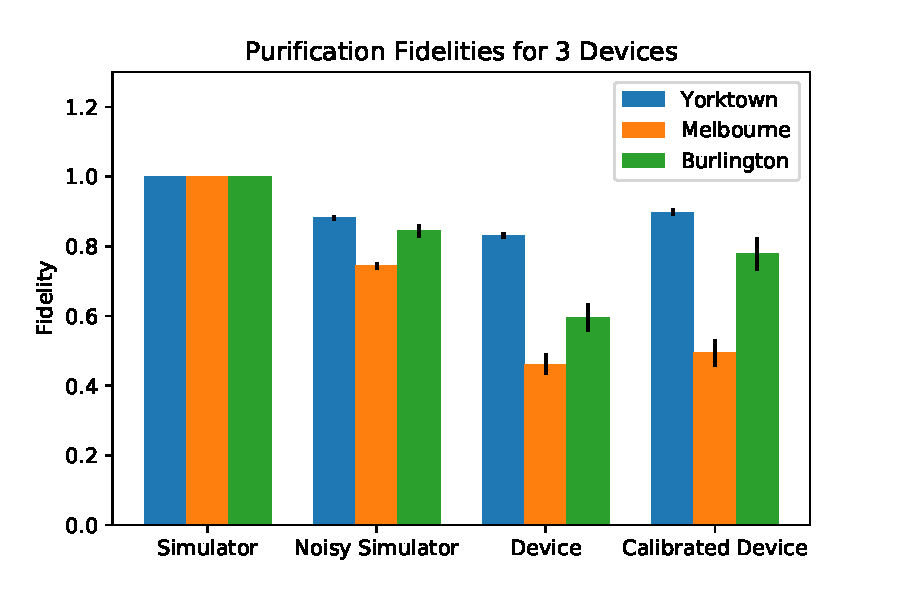
\includegraphics[width=0.48\textwidth]{images/results/purification_histogram.pdf}
	\caption{Fidelity results for the Purification protocol. Error bars are
    estimated taking the variance over 15 runs, where an average of 960 shots
    per run yield the desired entangled state.}
	\label{fig:purification_histogram}
\end{figure}

Now we will turn our attention to the Purification protocol, a circuit of great
use in quantum communication as noisy, imperfect entanglement can be improved on
through sifting the outcomes of measurements on a subset of received entangled
pairs. The statistics for this circuit are unique, because the purification
protocol relies on choosing the right outcomes (i.e. measuring the $\ket{11}$
state on the two measured qubits), which has a certain probability that depends
on the input fidelity of the entangled pairs. In the case where the input
fidelity to $\ket{\Phi^+}$ is 0.75, we expect the successful measurement outcome
a mere 12.5\% of the time. This means, out of the 122,880 shots we perform, only
an average of 15,360 will be successful.

\begin{figure}[h!]
	\begin{subfigure}{.5\textwidth}
    \centering
		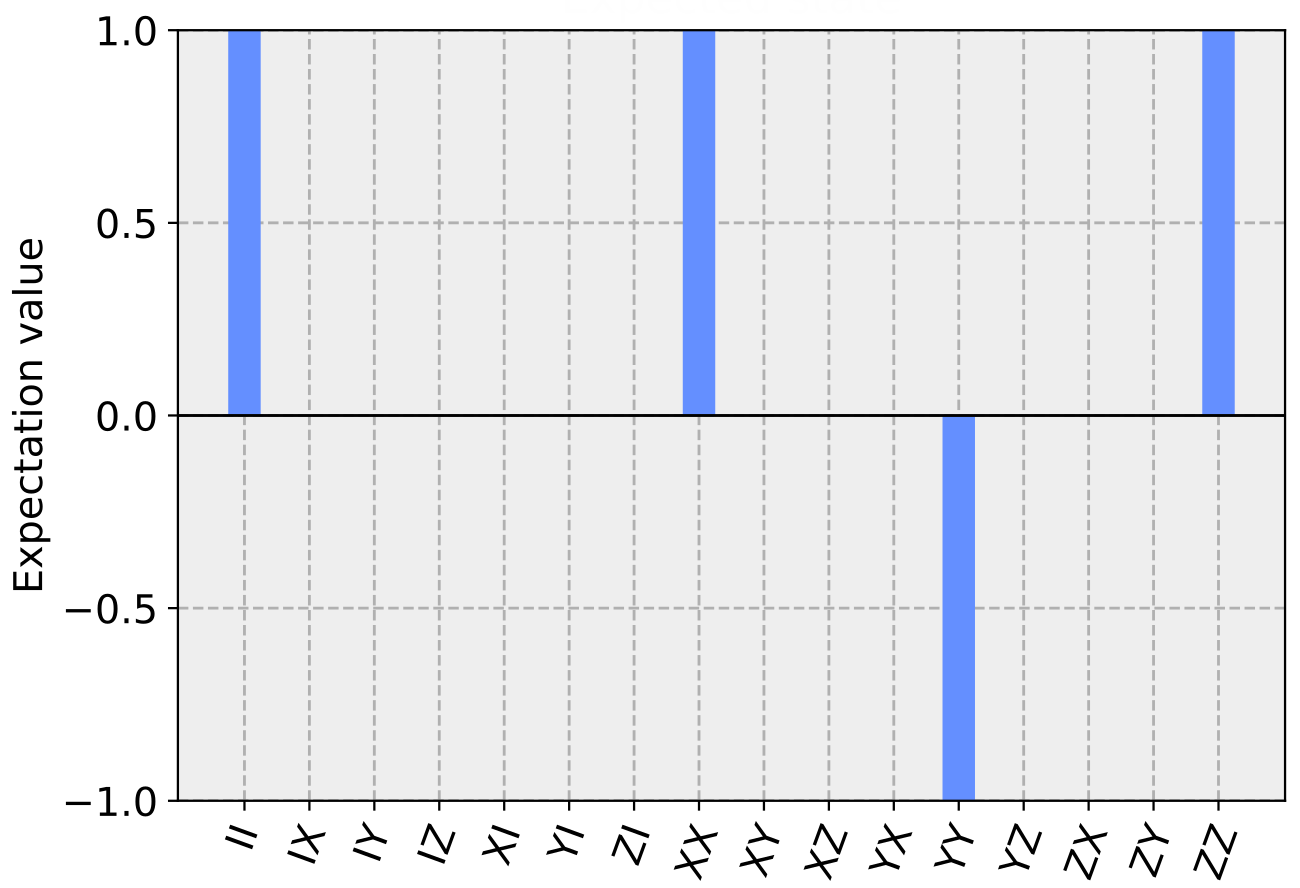
\includegraphics[width=.8\linewidth]{images/results/swap_pauli_sim.png}
		\caption{The expected Pauli set.}
		\label{fig:pur_pauli_sim}
	\end{subfigure} \newline
	\begin{subfigure}{.5\textwidth}
    \centering
		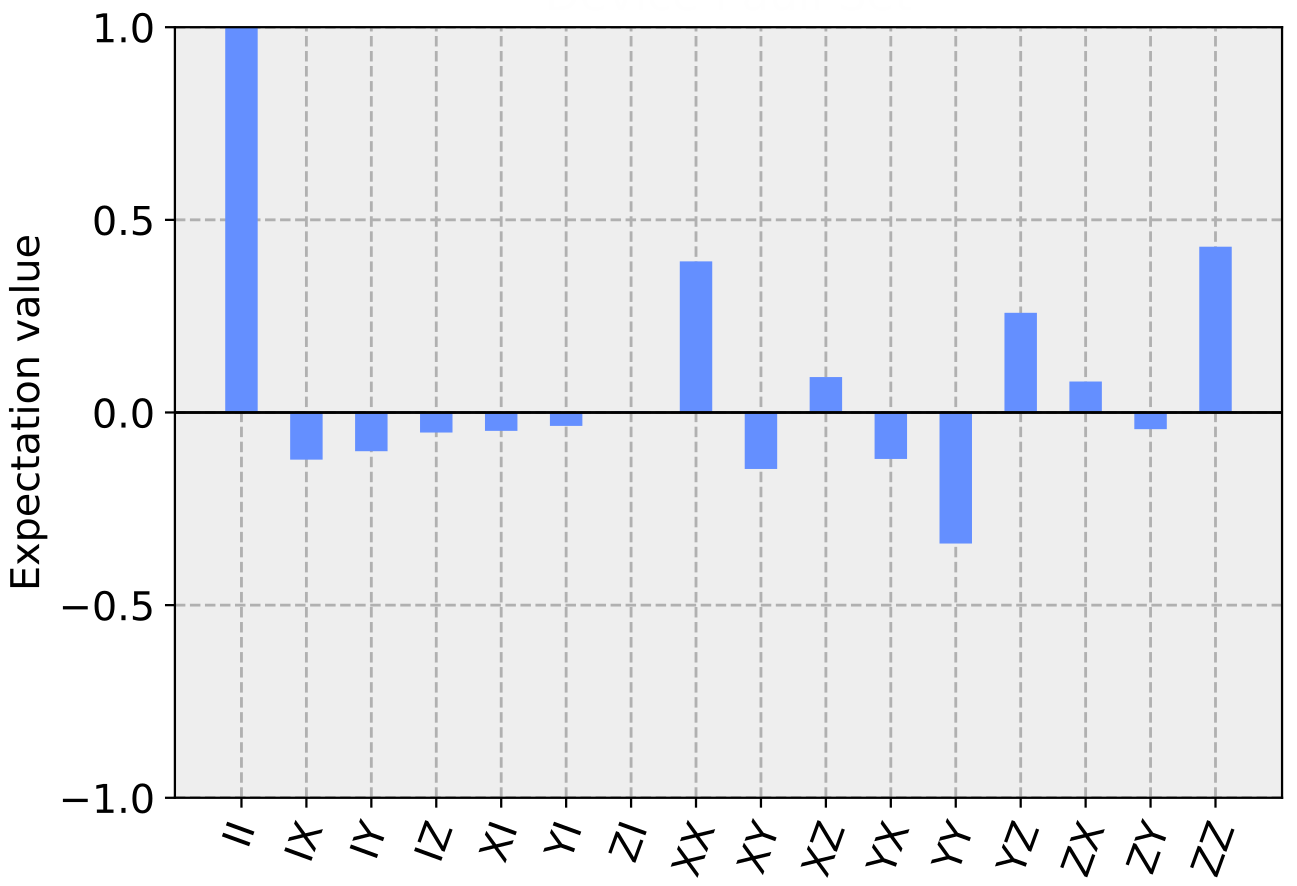
\includegraphics[width=.8\linewidth]{images/results/pur_pauli_dev.png}
		\caption{The output Pauli set for the device.}
		\label{fig:pur_pauli_dev}
	\end{subfigure} \newline
	\begin{subfigure}{.5\textwidth}
    \centering
		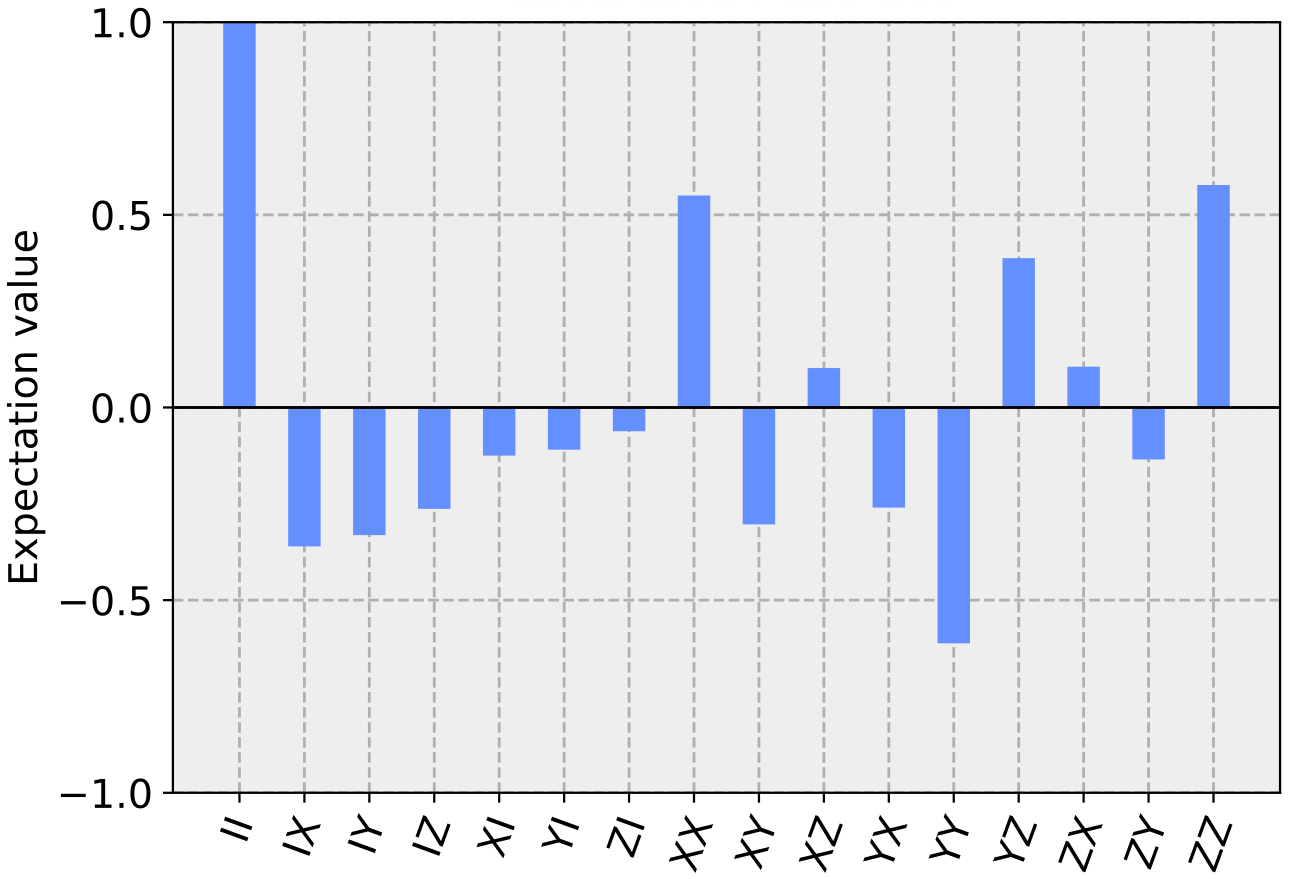
\includegraphics[width=.8\linewidth]{images/results/pur_pauli_cal.png}
		\caption{The calibrated device Pauli set.}
		\label{fig:pur_pauli_cal}
	\end{subfigure}
	\caption{The Pauli sets for the expected state and the output of the raw and
    calibrated device. Data here are taken from the Burlington device, with an
    average of 15,360 shots (12.5\% of 122,880).}
	\label{fig:purification_paulis}
\end{figure}

The poorer performance of the Burlington device (as compared to Yorktown)
evidenced in Fig. \ref{fig:purification_histogram} can be explained by the fact
that, again, twice as many CNOT gates are required for Burlington (15 gates)
than for either Melbourne or Yorktown (7 gates each). What is harder to explain
is Melbourne's extremely poor performance. The circuit is implemented on qubits
0, 1, 2 and 14 on Melbourne, so the especially noisy qubit 13 is left out of the
system. Our current understanding of the connections and gate fidelities for
these backends does not present an immediate explanation for this large dip in
the Melbourne fidelities. Further work would be required to understand where
exactly the error is coming from. It seems clear that the Noisy Simulator model
is likewise incapable of capturing the error in Melbourne, given the large
discrepancy between the device and noisy simulator results.

As with the other circuits, we can compare the Pauli sets of the expected state
with the raw and calibrated outputs of the device. The result is shown in Fig.
\ref{fig:purification_paulis}. The raw output, from Burlington, is reflective of
the relatively low fidelity states from this particular backend. We see that the
correlated expectation values (the $\langle XX \rangle$, $\langle YY \rangle$
and $\langle ZZ \rangle$) grow appreciably from the raw to calibrated device
output. However, the \textit{all} expectation values grow, which suggests that
the increase in the average fidelities from readout calibration may be partly
spurious. The expected state should have no individual character in the two
qubits, and the readout calibration as it is done here may be too blunt an
approach to readout correction to be very effective in this case.

Nonetheless, with this protocol, it is possible to attain fidelities far above
the input of 75\% (as high as 83.1\% for the raw device on Yorktown, and 89.8\%
after calibration). The distribution of entanglement, a key prerequisite for the
creation of quantum networks, is much easier even with very poor input states.
The only caveat being that one needs a very large number of poorly entangled
states to start with, in order to make any reasonably high number of Bell states.

\subsection{Grover's Algorithm}
Lastely, we will turn to Grover's algorithm, a protocol which can find a black box input with high probability. The main results can be found in figure \ref{fig:grover_histogram}.
\begin{figure}[h!]
	\centering
	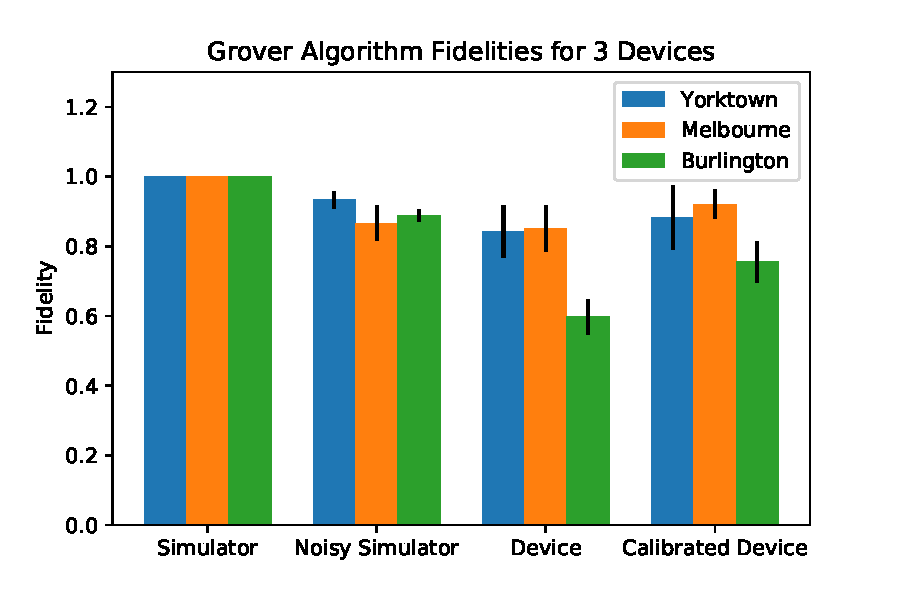
\includegraphics[width=0.48\textwidth]{images/results/grover_histogram.pdf}
	\caption{Fidelity results for Grover's algorithm. Error bars, showing
		one standard deviation, are estimated by taking the variance over 15 runs of
		8,192 shots each (a total of 122,880 shots).}
	\label{fig:grover_histogram}
\end{figure}
We can see that the simulation fidelities are 1, which is expected. The noisy simulator see to correspond well to the device and calibrated fidelities for Yorktown and Melbourne. These devices both show a similar (within statistical error) fidelity for the device and calibrated measurements. Again, the poor performance of Burlington can be easily seen. By comparison to the Yorktown and Melbourne fidelities, the Burlington fidelity is off by about 0.2. Also, the results show that a significant error is present in the measurement readout for Burlington. This can be seen by the increase after the correction. Where Yorktown and Melbourne fidelities increase by about 0.05, Burlington's fidelity increases by about 0.15. As the number of gates for each device is the same, the difference in fidelity is likely accounted to gate and measurement error. With Burlington having the lowest percentage in gate error, the measurement error of the device will probably be significant for Grover's algorithm.

Again, we can show the power of the measurement error correction in figure \ref{fig:grover_paulis}.
\begin{figure}[h!]
	\begin{subfigure}{.5\textwidth}
		\centering
		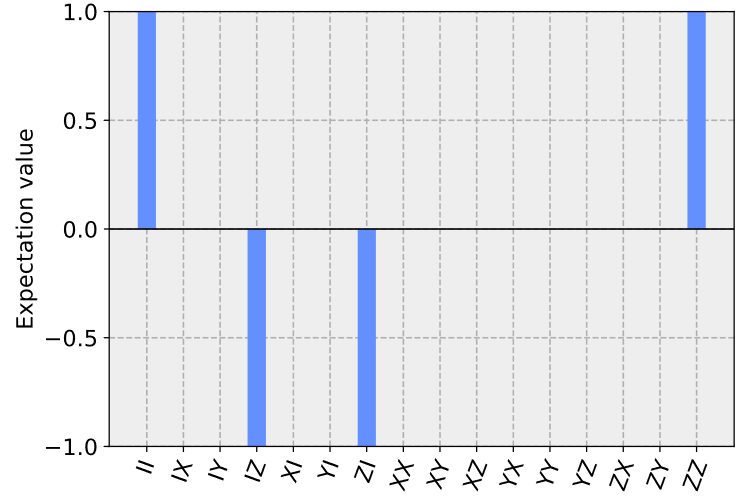
\includegraphics[width=.8\linewidth]{images/results/grov_pauli_sim.png}
		\caption{The expected Pauli set.}
		\label{fig:grov_pauli_sim}
	\end{subfigure} \newline
	\begin{subfigure}{.5\textwidth}
		\centering
		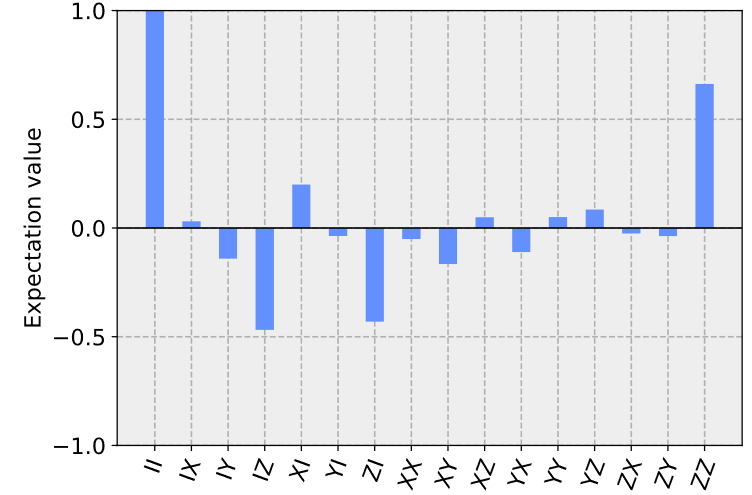
\includegraphics[width=.8\linewidth]{images/results/grov_pauli_dev.png}
		\caption{The output Pauli set for the device.}
		\label{fig:grov_pauli_dev}
	\end{subfigure} \newline
	\begin{subfigure}{.5\textwidth}
		\centering
		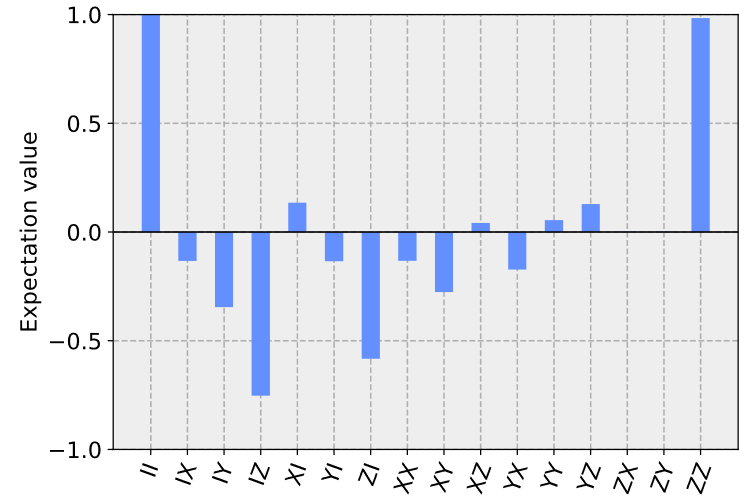
\includegraphics[width=.8\linewidth]{images/results/grov_pauli_cal.png}
		\caption{The calibrated device Pauli set.}
		\label{fig:grov_pauli_cal}
	\end{subfigure}
	\caption{The Pauli sets for Grover's algorithm, for the expected state and the output of the raw and
		calibrated device, for the -1 on the fourth position in $U$.  Data here are taken from the Burlington device.}
	\label{fig:grover_paulis}
\end{figure}
The output from the device shows a low fidelity pauli set. Where especially $\braket{IZ}$ and $\braket{ZI}$ have a small expectation value. After the correction we can see that the expectation value of $\braket{IZ}$ and $\braket{ZI}$ are significantly increased and the value of $\braket{ZZ}$ has become almost 1, as we expect from figure \ref{fig:grov_pauli_sim}. Unfortunately, the unwanted states also increase in expectation value, though this is overall a smaller increase. They still have a significant effect on the fidelity. But, it also shows the complete disappearance of unwanted states like $\braket{ZX}$ and $\braket{ZY}$. Nevertheless, the error correction is a helpful tool for increasing the fidelity of states, but has its limitations. This can also be visualized using the density matrices shown in figure \ref{fig:grov_density}.
\begin{figure}[h]
	\begin{subfigure}{.5\textwidth}
		\centering
		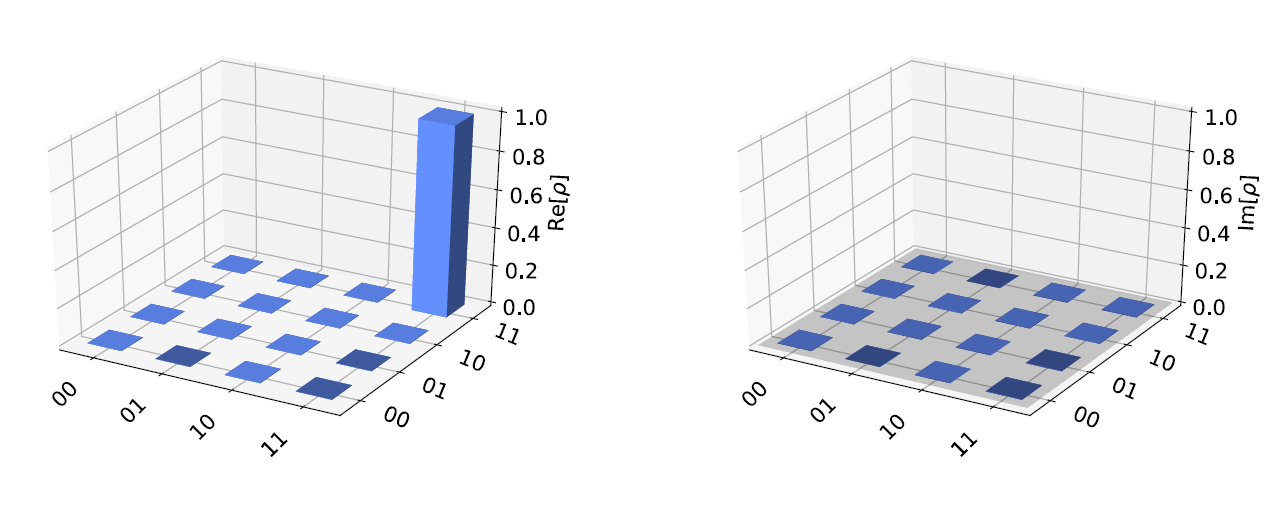
\includegraphics[width=.8\linewidth]{images/results/grov_density_sim.png}
		\caption{The expected Density matrix.}
		\label{fig:grov_density_sim}
	\end{subfigure} \newline
	\begin{subfigure}{.5\textwidth}
		\centering
		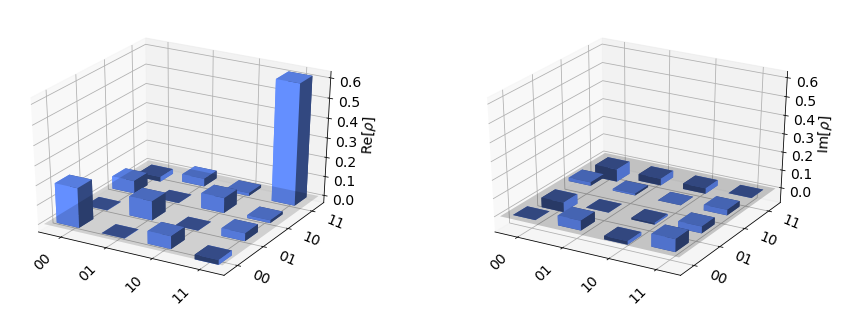
\includegraphics[width=.8\linewidth]{images/results/grov_density_dev.png}
		\caption{The output Density matrix for the device.}
		\label{fig:grov_density_dev}
	\end{subfigure} \newline
	\begin{subfigure}{.5\textwidth}
		\centering
		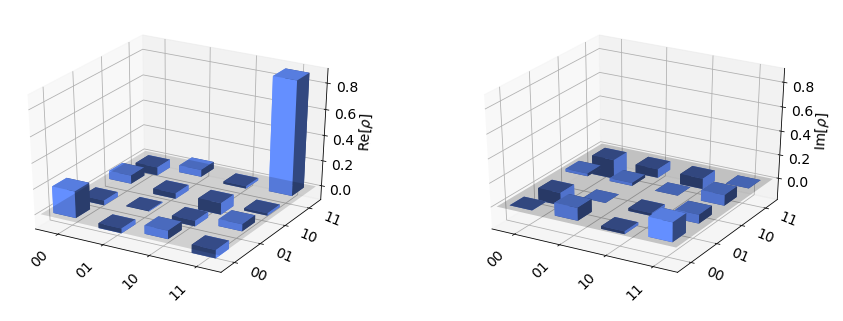
\includegraphics[width=.8\linewidth]{images/results/grov_density_cal.png}
		\caption{The calibrated device Density matrix.}
		\label{fig:grov_density_cal}
	\end{subfigure}
	\caption{The entanglement swapping density matrices for the ideal simulator,
		the device and the calibrated device, taken from Grover's algorithm. Data plotted here is taken for 8192 shots
		on the Burlington backend. }
	\label{fig:grov_density}
\end{figure}
Upon comparing figure \ref{fig:grov_density_dev} to \ref{fig:grov_density_cal}, we can clearly see the non relevant states, for example the 01 and 10 states, disappear from the (real part of the) density matrix.

%%% Local Variables:
%%% mode: latex
%%% TeX-master: "report"
%%% End: